\documentclass[
11pt, % The default document font size, options: 10pt, 11pt, 12pt
%codirector, % Uncomment to add a codirector to the title page
]{charter} 


% El títulos de la memoria, se usa en la carátula y se puede usar el cualquier lugar del documento con el comando \ttitle
\titulo{Sistema modular para monitoreo y control industrial con comunicación inalámbrica y capacidades de automatización embebida} 

% Nombre del posgrado, se usa en la carátula y se puede usar el cualquier lugar del documento con el comando \degreename
\posgrado{Carrera de Especialización en Sistemas Embebidos} 
%\posgrado{Carrera de Especialización en Internet de las Cosas} 
%\posgrado{Carrera de Especialización en Inteligencia Artificial}
%\posgrado{Maestría en Sistemas Embebidos} 
%\posgrado{Maestría en Internet de las cosas}

% Tu nombre, se puede usar el cualquier lugar del documento con el comando \authorname
% IMPORTANTE: no omitir titulaciones ni tildación en los nombres, también se recomienda escribir los nombres completos (tal cual los tienen en su documento)
\autor{Ing. Kirschner Lucas Sebastián}

% El nombre del director y co-director, se puede usar el cualquier lugar del documento con el comando \supname y \cosupname y \pertesupname y \pertecosupname
\director{Mgtr. Ing. Fernández Guillermo Alfredo}
\pertenenciaDirector{FIO - UNaM} 
\codirector{} % para que aparezca en la portada se debe descomentar la opción codirector en los parámetros de documentclass
\pertenenciaCoDirector{FIUBA}

% Nombre del cliente, quien va a aprobar los resultados del proyecto, se puede usar con el comando \clientename y \empclientename
\cliente{Representante de PyME industrial del sector manufacturero}
\empresaCliente{Industria tipo con bajo nivel de automatización}
 
\fechaINICIO{29 de abril de 2025}		%Fecha de inicio de la cursada de GdP \fechaInicioName
\fechaFINALPlan{17 de junio de 2025} 	%Fecha de final de cursada de GdP
\fechaFINALTrabajo{27 de abril de 2026}	%Fecha de defensa pública del trabajo final


\begin{document}

\maketitle
\thispagestyle{empty}
\pagebreak


\thispagestyle{empty}
{\setlength{\parskip}{0pt}
\tableofcontents{}
}
\pagebreak


\section*{Registros de cambios}
\label{sec:registro}


\begin{table}[ht]
\label{tab:registro}
\centering
\begin{tabularx}{\linewidth}{@{}|c|X|c|@{}}
\hline
\rowcolor[HTML]{C0C0C0} 
Revisión & \multicolumn{1}{c|}{\cellcolor[HTML]{C0C0C0}Detalles de los cambios realizados} & Fecha      \\ \hline
0      & Creación del documento                                 &\fechaInicioName \\ \hline
1      & Se completa hasta el punto 5 inclusive                & {12} de {mayo} de 2025 \\ \hline
%2      & Se completa hasta el punto 9 inclusive
%		  Se puede agregar algo más \newline
%		  En distintas líneas \newline
%		  Así                                                    & {día} de {mes} de 202X \\ \hline
%3      & Se completa hasta el punto 12 inclusive                & {día} de {mes} de 202X \\ \hline
%4      & Se completa el plan	                                 & {día} de {mes} de 202X \\ \hline

% Si hay más correcciones pasada la versión 4 también se deben especificar acá

\end{tabularx}
\end{table}

\pagebreak



\section*{Acta de constitución del proyecto}
\label{sec:acta}

\begin{flushright}
Buenos Aires, \fechaInicioName
\end{flushright}

\vspace{2cm}

Por medio de la presente se acuerda con el \authorname\hspace{1px} que su Trabajo Final de la \degreename\hspace{1px} se titulará ``\ttitle'' y consistirá en el desarrollo de un sistema distribuido conformado por una estación central y múltiples estaciones remotas, para facilitar la adquisición de datos de campo, el control de actuadores y la comunicación eficiente en entornos industriales donde las soluciones cableadas resultan poco prácticas o costosas. El trabajo tendrá un presupuesto preliminar de 680 horas y un costo estimado de \$ 11.000.000,00, con fecha de inicio el \fechaInicioName\hspace{1px} y fecha de presentación pública el \fechaFinalName.

Se adjunta a esta acta la planificación inicial.

\vfill

% Esta parte se construye sola con la información que hayan cargado en el preámbulo del documento y no debe modificarla
\begin{table}[ht]
\centering
\begin{tabular}{ccc}
\begin{tabular}[c]{@{}c@{}}Dr. Ing. Ariel Lutenberg \\ Director posgrado FIUBA\end{tabular} & \hspace{2cm} & \begin{tabular}[c]{@{}c@{}}\clientename \\ \empclientename \end{tabular} \vspace{2.5cm} \\ 
\multicolumn{3}{c}{\begin{tabular}[c]{@{}c@{}} \supname \\ Director del Trabajo Final\end{tabular}} \vspace{2.5cm} \\
\end{tabular}
\end{table}




\section{1. Descripción técnica-conceptual del proyecto a realizar}
\label{sec:descripcion}

El proyecto consiste en el desarrollo de un sistema modular para monitoreo y control industrial, con capacidades de automatización embebida y comunicación inalámbrica. Se trata de un emprendimiento personal, motivado por la necesidad detectada en industrias con baja adopción tecnológica y limitada conectividad cableada, que requieren soluciones ágiles, adaptables y robustas para mejorar sus procesos productivos.

En el contexto actual, muchos sistemas de automatización industrial están diseñados para instalaciones específicas. Sus arquitecturas suelen ser rígidas y presentan escasa capacidad de adaptación a entornos cambiantes o geográficamente dispersos. Las soluciones tradicionales dependen en gran medida de infraestructura cableada, lo cual representa una limitación significativa en entornos donde el tendido de cables es costoso o impracticable. En contraste, este proyecto se enfoca en brindar una alternativa distribuida y escalable, basada en tecnologías modernas de microcontroladores, comunicación inalámbrica y diseño modular.

La solución propuesta contempla una arquitectura distribuida compuesta por una estación central y múltiples estaciones remotas. La estación central se construirá en torno a un microcontrolador de altas prestaciones (por ejemplo, ARM Cortex-M7 o M33), con capacidad para ejecutar múltiples tareas con restricciones temporales mediante un sistema operativo en tiempo real (\textit{Real-Time Operating System}, RTOS). Integrará una interfaz Ethernet para conexión con sistemas de supervisión y control, tales como plataformas \textit{Supervisory Control and Data Acquisition} (SCADA), y una interfaz inalámbrica de alta confiabilidad para comunicarse con las estaciones remotas. También contará con un reloj en tiempo real (\textit{Real-Time Clock}, RTC) para mantener el registro horario, y se evaluará el uso de \textit{Power over Ethernet} (PoE) como alternativa de alimentación.

Las estaciones remotas estarán equipadas con microcontroladores de menores recursos (como ARM Cortex-M3 o M4), orientados a la adquisición de señales y a la activación de actuadores en campo. Contarán con entradas y salidas digitales industriales, adecuadas para la conexión de sensores discretos y dispositivos como relés o contactores, así como una interfaz de comunicación industrial, como por ejemplo RS485, que permita la integración con diversos equipos del entorno. La comunicación con la estación central se realizará mediante un enlace inalámbrico confiable. Estas estaciones estarán diseñadas para operar en entornos exigentes, alimentadas desde la red eléctrica de 220 V, con la posibilidad de integrar baterías de respaldo para asegurar continuidad operativa.

Desde el punto de vista del software, se implementará una arquitectura por capas que permita separar claramente las funciones de bajo nivel (controladores, comunicación, gestión de entradas/salidas) de la lógica de aplicación. Se proveerá una interfaz de programación de aplicaciones (\textit{Application Programming Interface}, API) que facilite el desarrollo de soluciones específicas sobre la plataforma base. Este enfoque modular permitirá escalar el sistema según las necesidades, incorporar nuevas estaciones o funcionalidades sin rediseñar el conjunto, y facilitar su mantenimiento y extensión futura.

La propuesta se destaca por su flexibilidad, escalabilidad y adaptabilidad. Frente a las soluciones actuales, que suelen ser cerradas y costosas, este proyecto plantea un sistema abierto y personalizable, orientado a pequeñas y medianas industrias que requieren soluciones específicas sin incurrir en altos costos de integración.

\newpage
La figura \ref{fig:diagBloques} presenta el diagrama en bloques del sistema propuesto, el cual resume visualmente la arquitectura distribuida planteada. Se distinguen claramente la estación central, con su microcontrolador de altas prestaciones, las interfaces de comunicación (Ethernet e inalámbrica) y las opciones de alimentación (PoE o red eléctrica), y las estaciones remotas, dotadas de entradas y salidas digitales industriales, interfaz inalámbrica y comunicación serie robusta para dispositivos de campo.

\begin{figure}[htpb]
\centering 
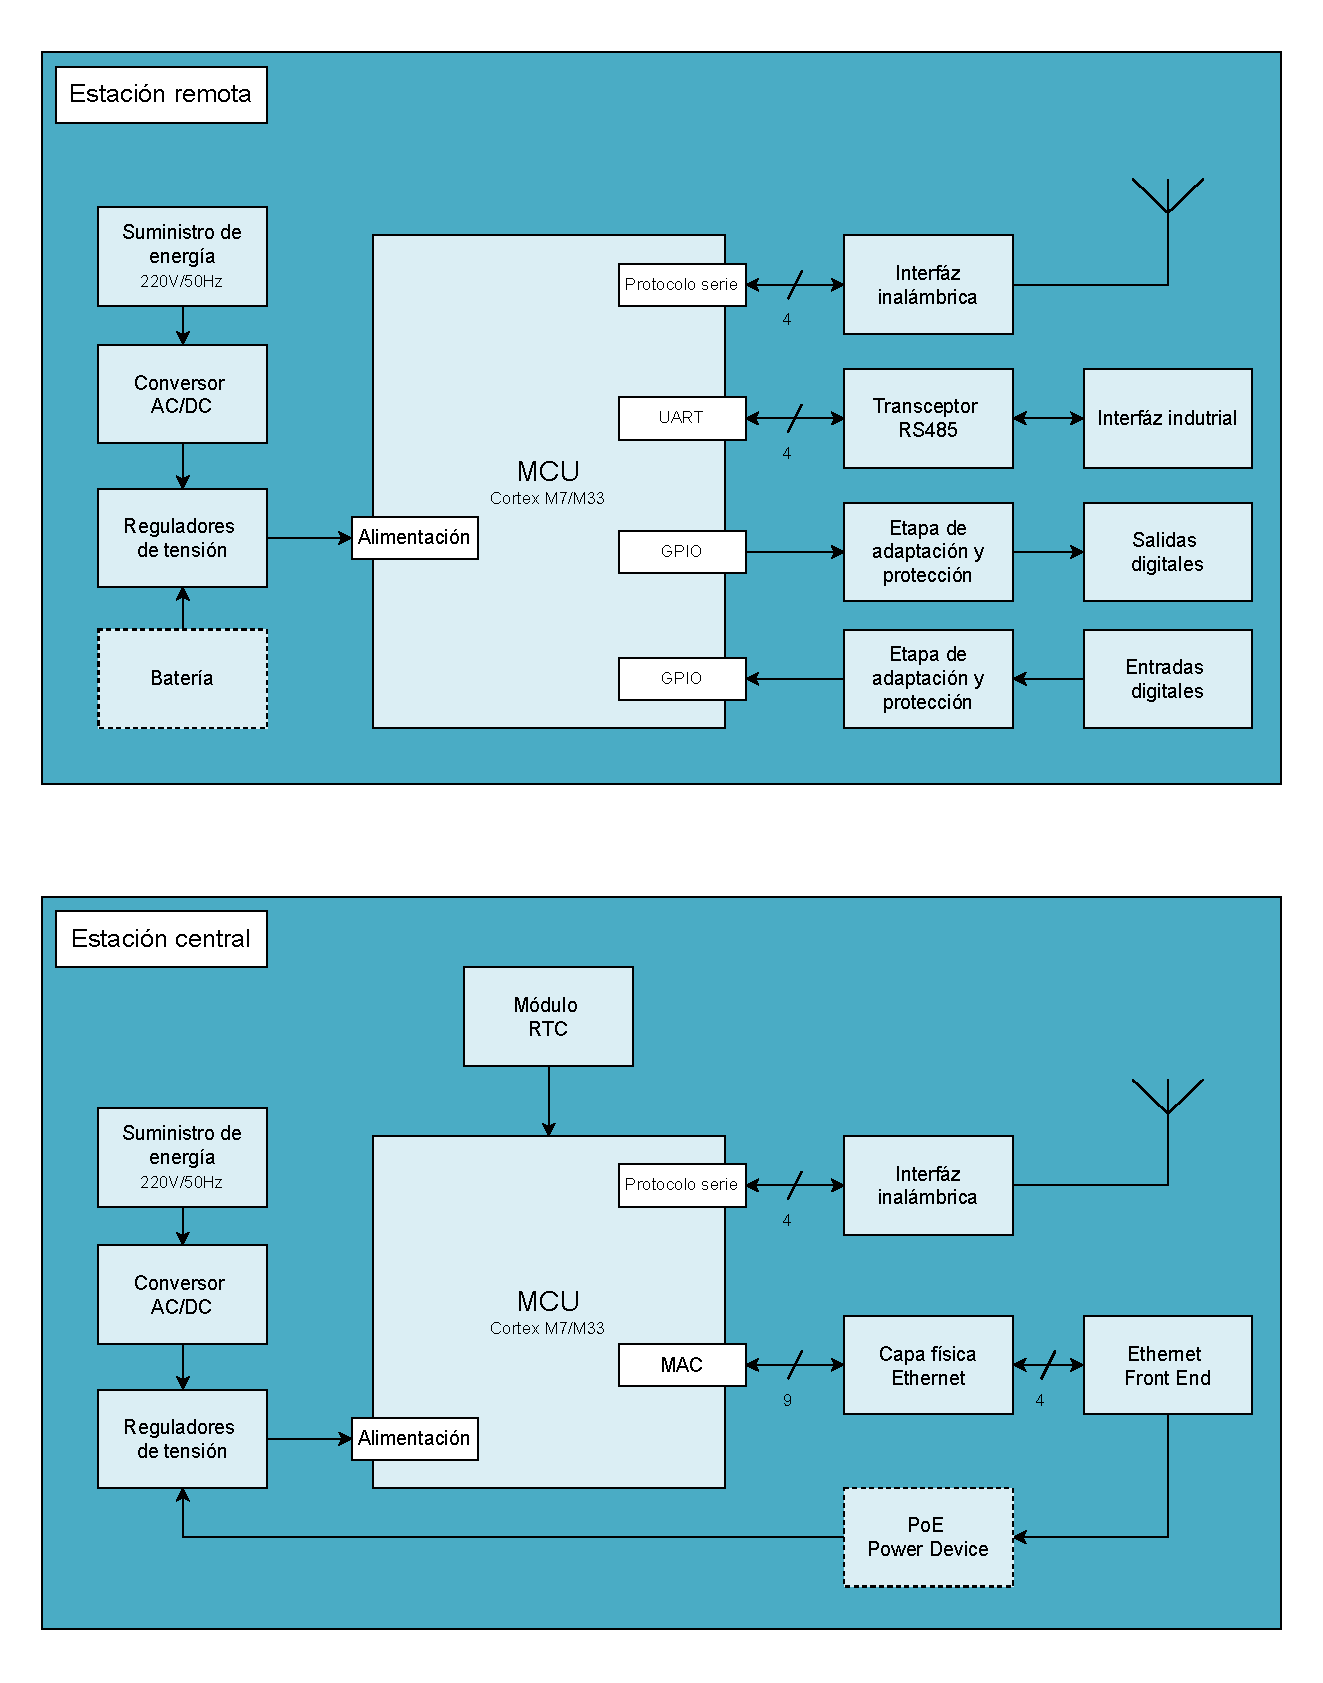
\includegraphics[width=.9\textwidth]{./Figuras/diagBloques.pdf}
\caption{Diagrama en bloques del sistema.}
\label{fig:diagBloques}
\end{figure}

\section{2. Identificación y análisis de los interesados}
\label{sec:interesados}

A continuación, se identifican los principales interesados del proyecto, detallando sus roles, vínculos con el desarrollo y nivel de participación esperado.

\begin{table}[H]
%\caption{Identificación de los interesados}
%\label{tab:interesados}
\begin{tabularx}{\linewidth}{@{}|l|X|X|X|@{}}
\hline
\rowcolor[HTML]{C0C0C0} 
Rol           & Nombre y Apellido & Organización 	& Puesto 	\\ \hline
%Auspiciante   &                   &              	&        	\\ \hline
Cliente       & -      &\empclientename	& \clientename        	\\ \hline
%Impulsor      & Kirschner Lucas Sebastián & -      	& Emprendedor y promotor de la iniciativa \\ \hline
Responsable   & \authorname       & FIUBA        	& Alumno 	\\ \hline
%Colaboradores &                   &              	&        	\\ \hline
Orientador    & \supname	      & \pertesupname 	& Director del Trabajo Final \\ \hline
%Equipo        & miembro1 \newline 
%				miembro2          &              	&        	\\ \hline
Opositores    & -                 & Fabricantes e integradores tradicionales de PLC & Actores con intereses en soluciones cableadas tradicionales \\ \hline
Usuario final & - 				  & Industria genérica & Operadores y encargados de mantenimiento \\ \hline
\end{tabularx}
\end{table}
 
\begin{itemize}
	\item Cliente: Representado por industrias con baja incorporación tecnológica y limitada infraestructura de conectividad. Este tipo de organización busca soluciones que le permitan modernizar sus procesos productivos sin necesidad de realizar grandes inversiones en cableado o infraestructura física. Valora la simplicidad en la implementación, la escalabilidad y la robustez de los sistemas.
	
	%\item Impulsor: Lucas Sebastián Kirschner, autor del proyecto y profesional del área, identifica la necesidad del sector y promueve una solución técnica innovadora basada en su experiencia en sistemas embebidos. En este rol, impulsa el desarrollo, búsqueda de valor y validación de la propuesta, combinando visión técnica y estratégica.
	
	\item Responsable: El autor del proyecto, Ing. Lucas Sebastián Kirschner, asume la responsabilidad sobre el mismo. Tiene a su cargo el diseño, implementación, validación y documentación del sistema, así como la planificación y ejecución del trabajo dentro de los plazos establecidos.
	
	\item Orientador: El Mgtr. Ing. Guillermo Alfredo Fernández es profesor titular e investigador de la Facultad de Ingeniería de la Universidad Nacional de Misiones (FIO - UNaM), con una reconocida trayectoria en sistemas embebidos aplicados a energías renovables y automatización. Su rol es fundamental para validar las decisiones técnicas, guiar metodológicamente el desarrollo y asegurar el rigor académico del trabajo final.
	
	\item Opositores: Fabricantes de PLC convencionales e integradores de soluciones cableadas que podrían ver afectada su posición en el mercado ante la aparición de propuestas modulares, económicas y de implementación más ágil como la que plantea este proyecto. Esta oposición potencial se da principalmente en entornos donde la adopción de nuevas tecnologías no forma parte del modelo de negocio tradicional.
	
	\item Usuario final: Personal técnico de planta, incluyendo operarios, encargados de mantenimiento y supervisores de proceso. Interactuarán con el sistema para monitorear variables de proceso y controlar dispositivos industriales. Se prioriza la facilidad de uso, confiabilidad operativa y adaptación a diferentes entornos industriales.
\end{itemize}

\newpage
\section{3. Propósito del proyecto}
\label{sec:proposito}

Desarrollar una solución modular y escalable que permita monitorear y controlar procesos industriales en entornos con baja infraestructura de conectividad, mediante una arquitectura distribuida que combine estaciones centrales y remotas interconectadas por enlaces inalámbricos confiables. La iniciativa surge como respuesta a la necesidad de automatización en industrias que presentan limitaciones técnicas, económicas o geográficas para implementar sistemas cableados convencionales, y busca facilitar la recolección de datos de campo, la activación de actuadores y la implementación de lógica de control adaptada a cada caso. %Mediante el diseño de hardware robusto y firmware con capas de abstracción bien definidas, se espera reducir barreras técnicas para el desarrollo de aplicaciones específicas, optimizar el mantenimiento de equipos, mejorar la eficiencia operativa y ofrecer una herramienta flexible que se adapte a distintas escalas de implementación industrial.

\section{4. Alcance del proyecto}
\label{sec:alcance}

El proyecto incluye:
\begin{itemize}
	\item El diseño y construcción de un prototipo funcional de la estación central, basada en un microcontrolador de altas prestaciones con capacidad para ejecutar un sistema operativo de tiempo real (RTOS).
	\item El diseño y fabricación de al menos dos prototipos funcionales de estaciones remotas, con interfaces para la conexión de sensores y actuadores industriales.
	\item El diseño e implementación de la arquitectura de alimentación, contemplando el uso de PoE como opción de suministro para la estación central y la incorporación de baterías de respaldo en las estaciones remotas.
	\item El desarrollo del firmware de bajo nivel para la inicialización de periféricos, gestión de comunicaciones y manejo de entradas/salidas en ambas estaciones.
	\item La implementación de una API modular que abstraiga la complejidad del hardware y facilite la adaptación del sistema a distintos procesos industriales.
	\item La validación funcional de los módulos mediante pruebas controladas que simulen condiciones reales del entorno industrial.
\end{itemize}

El presente proyecto no incluye:
\begin{itemize}
	\item El desarrollo de una interfaz gráfica de supervisión (HMI/SCADA).
	\item La integración con sistemas productivos reales de empresas externas.
	\item La incorporación de inteligencia artificial embebida, aunque se considera su viabilidad para futuras etapas.
	\item El diseño de encapsulados o gabinetes industriales, más allá de criterios básicos de disposición y conexión.
	\item La certificación del producto para entornos industriales normados.
	\item La obtención de un sistema final manufacturable, dado que el proyecto se limita a la construcción y validación de prototipos funcionales.
\end{itemize}

\section{5. Supuestos del proyecto}
\label{sec:supuestos}

Para el desarrollo del presente proyecto se supone que:

\begin{itemize}
	\item Se dispondrá de tiempo suficiente por parte del responsable para cumplir con las actividades planificadas.
	\item Se podrán adquirir los componentes electrónicos necesarios en el mercado local o internacional, sin demoras significativas ni incrementos abruptos de costos.
	\item No se presentarán restricciones legales, regulatorias o normativas que impidan la realización del proyecto o el uso de tecnologías previstas.
	\item No habrá una devaluación abrupta que comprometa la adquisición de insumos clave o el cumplimiento del presupuesto estimado.
	\item La tecnología inalámbrica seleccionada será factible de implementar con los recursos disponibles y adecuada para el tipo de comunicación requerida entre estaciones.
	\item El entorno de prueba seleccionado permitirá validar adecuadamente el funcionamiento del sistema en condiciones representativas.
	\item Se contará con acceso a herramientas y bibliografía técnica suficiente para el diseño, implementación y validación del sistema.
	\item El desarrollo del firmware y la arquitectura modular prevista podrán implementarse con herramientas de software disponibles sin incurrir en costos adicionales significativos.
\end{itemize}

\section{6. Requerimientos}
\label{sec:requerimientos}

\begin{enumerate}
	\item Requerimientos de hardware:
		\begin{enumerate}
			\item El sistema deberá contar con una estación central basada en un microcontrolador ARM Cortex-M7 (o superior), con al menos 512 KB de RAM y 2 MB de Flash.
			\item Las estaciones remotas deberán emplear microcontroladores ARM Cortex-M3/M4 o similar, con al menos 64 KB de RAM y 256 KB de Flash.
			\item La interfaz RS485 deberá cumplir con la norma TIA/EIA-485-A, soportando velocidades de hasta 115200 baudios en distancias de hasta 100 m.
			\item Cada estación remota deberá contar con entradas digitales compatibles con sensores industriales de 24 V con colector abierto.
			\item Las salidas digitales deberán soportar cargas de al menos 30 V y 500 mA, con aislamiento galvánico mediante optoacopladores o relés.
			\item Las estaciones deberán alimentarse desde la red eléctrica de 220 V/50 Hz, mediante conversores internos.
			\item La estación central deberá incluir un RTC con respaldo energético para mantener fecha y hora ante cortes de energía.
			\item Opcionalmente, las estaciones remotas podrán alimentarse mediante baterías internas cuando no se disponga de acceso directo a la red eléctrica o se desee simplificar su instalación en ubicaciones aisladas.
		\end{enumerate}
		
	\item Requerimientos de comunicación:
		\begin{enumerate}
			\item La comunicación entre estación central y estaciones remotas se realizará mediante un protocolo inalámbrico que asegure un alcance mínimo de 20 m en interiores, utilizando antenas incorporadas.
			\item El sistema deberá permitir la conexión de hasta 16 estaciones remotas a una misma estación central.
			\item La estación central deberá contar con interfaz Ethernet 10/100 Mbps para la conexión con sistemas SCADA o de supervisión.
			\item El protocolo inalámbrico deberá contemplar acuse de recibo y retransmisión de mensajes no confirmados.
		\end{enumerate}
		
	\item Requerimientos de firmware:
		\begin{enumerate}
			\item El firmware deberá estar basado en arquitectura en capas, con separación entre drivers, middleware y lógica de aplicación.
			\item La estación central deberá ejecutar un sistema operativo de tiempo real (RTOS) con soporte para tareas concurrentes.
			\item Se deberá implementar una API estandarizada para el acceso a sensores y actuadores, tanto locales como remotos.
			\item El desarrollo deberá utilizar control de versiones con Git.
			\item Se emplearán buenas prácticas de programación modular y segura, inspiradas en lineamientos como MISRA-C.
		\end{enumerate}
		
	\item Requerimientos de documentación:
		\begin{enumerate}
			\item Se deberá entregar documentación técnica del hardware: esquemáticos, lista de materiales y archivos de fabricación (gerbers).
			\item La API del sistema deberá documentarse utilizando una herramienta de documentación automática como Doxygen.
			\item Opcionalmente, se podrá incluir un manual de instalación y puesta en marcha orientado al usuario final.
		\end{enumerate}
		
	\item Requerimientos de validación y pruebas:
		\begin{enumerate}
			\item Se deberán realizar pruebas funcionales que verifiquen la correcta lectura de sensores y la activación de salidas digitales, utilizando equipos de laboratorio.
			\item Se deberán validar las funciones de comunicación inalámbrica y cableada mediante ensayos controlados en condiciones reproducibles.
			\item Se deberá confirmar la integridad funcional del sistema en escenarios que simulen condiciones típicas de operación.
		\end{enumerate}
		
	\item Requerimientos normativos:
		\begin{enumerate}
			\item El diseño del hardware deberá cumplir con las normas de seguridad eléctrica aplicables a equipos de baja tensión (por ej. IEC 61010 o IRAM equivalente).
			\item Las placas de circuito impreso deberán diseñarse siguiendo la normativa IPC correspondiente (ej. IPC-2221, IPC-7351).
			\item La documentación técnica deberá estructurarse siguiendo buenas prácticas industriales.
		\end{enumerate}
		

\end{enumerate}

\section{7. Historias de usuarios (\textit{Product backlog})}
\label{sec:backlog}

Las siguientes historias de usuarios describen funcionalidades deseables para distintos perfiles involucrados en la utilización, integración o instalación del sistema. Cada historia fue ponderada según su complejidad estimada, utilizando el enfoque de \textit{story points}, basado en la suma de tres dimensiones:

\begin{itemize}
	\item Dificultad: nivel de complejidad técnica para implementar la historia.
	\item Tiempo de implementación: cantidad de trabajo estimado para completarla.
	\item Incertidumbre: grado de riesgo técnico o falta de información.
\end{itemize}

Cada dimensión toma un valor entre 1 (bajo), 2 (medio) y 3 (alto), dando lugar a una suma total que se traduce en los \textit{story points} asociados. La prioridad relativa de cada historia (1 a 5) indica su importancia funcional respecto del resto.

\begin{enumerate}
	\item Como técnico instalador, quiero que las estaciones remotas dispongan de conectores industriales normalizados y borneras identificadas, para realizar una instalación rápida y sin errores.\\
	\textit{Story points: 4} (dificultad: 1, tiempo de implementación: 1, incertidumbre: 2).
	
	\item Como ingeniero de mantenimiento, quiero que el sistema sea modular y permita reemplazar estaciones remotas sin reconfigurar la estación central, para facilitar el mantenimiento correctivo.\\
	\textit{Story points: 7} (dificultad: 2, tiempo de implementación: 2, incertidumbre: 3).
	
	\item Como desarrollador de sistemas embebidos, quiero disponer de una API clara y documentada para programar la lógica de control del sistema, para poder implementar distintas aplicaciones sin modificar las capas base.\\
	\textit{Story points: 7} (dificultad: 2, tiempo de implementación: 3, incertidumbre: 2).
	
	\item Como dueño de la empresa, quiero que los equipos desarrollados puedan certificarse según normas industriales comunes, para asegurar la compatibilidad con estándares del sector.\\
	\textit{Story points: 9} (dificultad: 3, tiempo de implementación: 3, incertidumbre: 3).
	
	\item Como operador de mantenimiento, quiero recibir alertas en caso de desconexión prolongada de una estación remota, para poder actuar de forma preventiva ante fallas de comunicación.\\
	\textit{Story points: 8} (dificultad: 3, tiempo de implementación: 3, incertidumbre: 2).
	
	\item Como usuario integrador del sistema, quiero poder configurar desde software el comportamiento de las estaciones remotas, para adaptar su funcionamiento a distintas aplicaciones industriales.\\
	\textit{Story points: 7} (dificultad: 2, tiempo de implementación: 3, incertidumbre: 2).
	
	\item Como desarrollador de firmware, quiero contar con ejemplos de referencia y librerías reutilizables, para acelerar el desarrollo de nuevas estaciones remotas.\\
	\textit{Story points: 7} (dificultad: 2, tiempo de implementación: 3, incertidumbre: 2).
\end{enumerate}

\section{8. Entregables principales del proyecto}
\label{sec:entregables}

\begin{itemize}
	\item Diagramas de circuitos esquemáticos de las estaciones central y remota.
	\item Listado de materiales (\textit{Bill of Materials}, BOM) de las estaciones central y remota.
	\item Diseño de los circuitos impresos (\textit{Printed Circuit Board}, PCB) y generación de archivos de fabricación (\textit{gerbers} y archivos de ensamblado).
	\item Prototipos funcionales de al menos una estación central y dos estaciones remotas.
	\item Código fuente del firmware para estación central y estaciones remotas.
	\item Documentación de la API.
	\item Memoria técnica del trabajo final.
\end{itemize}

\section{9. Desglose del trabajo en tareas}
\label{sec:wbs}

\begin{enumerate}
	\item Investigación preliminar (70 h)
	\begin{enumerate}
		\item Revisión del estado del arte de tecnologías inalámbricas para comunicación entre nodos (20 h).
		\item Revisión de normativas industriales vigentes (compatibilidad electromagnética, alimentación, comunicaciones, etc.) (10 h).
		\item Selección preliminar de microcontroladores para estación central y remotas. (15 h)
		\item Estudio de alternativas de interfaz RS485 (10 h).
		\item Revisión de opciones de alimentación y protección eléctrica para ambientes industriales (15 h).
	\end{enumerate}
	
	\item Desarrollo de hardware (210 h)
	\begin{enumerate}
		\item Revisión de proyectos similares: esquemas eléctricos, placas comerciales, kits de desarrollo, datasheets, notas de aplicación (20 h).
		\item Planteo de la estructura del sistema: definición de módulos, arquitectura general, diagrama de bloques, topología de conexión (15 h).
		\item Selección definitiva de componentes principales (15 h).
		\item Creación de librerías de componentes personalizados (\textit{footprints}, símbolos) (15 h).
		\item Diseño del esquemático eléctrico de la estación central (20 h).
		\item Diseño del esquemático eléctrico de las estaciones remotas (20 h).
		\item Ruteo del PCB de la estación central (25 h).
		\item Ruteo del PCB de las estaciones remotas (25 h).
		\item Generación de archivos \textit{gerbers}, BOM y archivos de ensamblado (pick and place, etc.) (10 h).
		\item Pedido de prototipos y compra de componentes (5 h).
		\item Armado de prototipos (20 h).
		\item Pruebas funcionales eléctricas y corrección de errores de hardware (20 h).
	\end{enumerate}
	\newpage
	\item Desarrollo de firmware (250 h)
	\begin{enumerate}
		\item Investigación y selección de un RTOS (25 h).
		\item Definición de la estructura modular del firmware (drivers, lógica de aplicación, comunicación, etc.) (15 h).
		\item Definición de la arquitectura del firmware de la estación central (20 h).
		\item Definición de la arquitectura del firmware de las estaciones remotas (20 h).
		\item Diseño e implementación de la API (35 h).
		\item Programación de drivers (35 h).
		\item Implementación del stack de comunicación RS485 (30 h).
		\item Implementación del stack TCP/IP (35 h).
		\item Desarrollo de funciones de adquisición, control de salidas y configuración remota (35 h).
		\item Documentación técnica del firmware y la API (20 h).
	\end{enumerate}
	
	\item Integración del sistema (70 h)
	\begin{enumerate}
		\item Integración de hardware y firmware en estación central (15 h).
		\item Integración de hardware y firmware en estaciones remotas (15 h).
		\item Integración del sistema inalámbrico: comunicación entre estaciones remotas y estación central. (25 h).
		\item Ajustes de firmware y hardware tras integración inicial (15 h).
	\end{enumerate}
	
	\item Pruebas de validación (50 h)
	\begin{enumerate}
		\item Diseño de casos de prueba funcionales y de comunicación (15 h).
		\item Ejecución de pruebas generales sobre el sistema completo (20 h).
		\item Evaluación del desempeño en condiciones simuladas (15 h).
	\end{enumerate}
	
	\item Cierre del proyecto (30 h)
	\begin{enumerate}
		\item Elaboración de la memoria técnica (20 h).
		\item Elaboración de la presentación final (10 h).
	\end{enumerate}
\end{enumerate}

Cantidad total de horas: 680 h

\section{10. Diagrama de Activity On Node}
\label{sec:AoN}

\begin{consigna}{red}
Armar el AoN a partir del WBS definido en la etapa anterior.

Una herramienta simple para desarrollar los diagramas es el Draw.io (\url{https://app.diagrams.net/}).
\href{https://app.diagrams.net}{Draw.io}


\begin{figure}[htpb]
\centering 
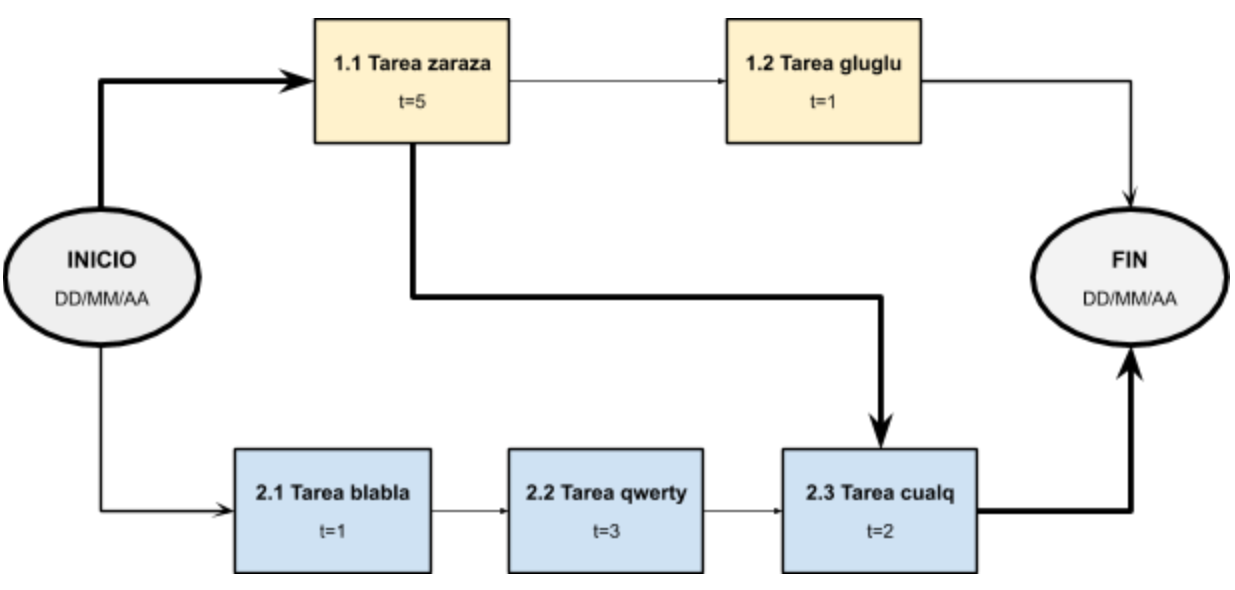
\includegraphics[width=.8\textwidth]{./Figuras/AoN.png}
\caption{Diagrama de \textit{Activity on Node}.}
\label{fig:AoN}
\end{figure}

Indicar claramente en qué unidades están expresados los tiempos.
De ser necesario indicar los caminos semi críticos y analizar sus tiempos mediante un cuadro.
Es recomendable usar colores y un cuadro indicativo describiendo qué representa cada color.

\end{consigna}

\section{11. Diagrama de Gantt}
\label{sec:gantt}

\begin{consigna}{red}
Existen muchos programas y recursos \textit{online} para hacer diagramas de Gantt, entre los cuales destacamos:

\begin{itemize}
\item Planner
\item GanttProject
\item Trello + \textit{plugins}. En el siguiente link hay un tutorial oficial: \\ \url{https://blog.trello.com/es/diagrama-de-gantt-de-un-proyecto}
\item Creately, herramienta online colaborativa. \\\url{https://creately.com/diagram/example/ieb3p3ml/LaTeX}
\item Se puede hacer en latex con el paquete \textit{pgfgantt}\\ \url{http://ctan.dcc.uchile.cl/graphics/pgf/contrib/pgfgantt/pgfgantt.pdf}
\end{itemize}

Pegar acá una captura de pantalla del diagrama de Gantt, cuidando que la letra sea suficientemente grande como para ser legible. 
Si el diagrama queda demasiado ancho, se puede pegar primero la ``tabla'' del Gantt y luego pegar la parte del diagrama de barras del diagrama de Gantt.

Configurar el software para que en la parte de la tabla muestre los códigos del EDT (WBS).\\
Configurar el software para que al lado de cada barra muestre el nombre de cada tarea.\\
Revisar que la fecha de finalización coincida con lo indicado en el Acta Constitutiva.

En la figura \ref{fig:gantt}, se muestra un ejemplo de diagrama de gantt realizado con el paquete de \textit{pgfgantt}. 
En la plantilla pueden ver el código que lo genera y usarlo de base para construir el propio.

Las fechas pueden ser calculadas utilizando alguna de las herramientas antes citadas. Sin embargo, el siguiente ejemplo
fue elaborado utilizando 
\href{https://docs.google.com/spreadsheets/d/1fBz8NhSpc4tkkhz3KjJCbh1nR_ltDkfEcZi4tZXduqs}{esta hoja de cálculo}.

Es importante destacar que el ancho del diagrama estará dado por la longitud del texto utilizado para las tareas 
(Ejemplo: tarea 1, tarea 2, etcétera) y el valor \textit{x unit}. Para mejorar la apariencia del diagrama, es necesario
ajustar este valor y, quizás, acortar los nombres de las tareas.

\begin{figure}[htpb]
  \begin{center}
    \begin{ganttchart}[
      time slot unit=day,
      time slot format=isodate,
      x unit=0.038cm,
      y unit title=0.7cm,
      y unit chart=0.6cm,
      milestone/.append style={xscale=4}
      ]{2021-03-05}{2021-12-16}
      \gantttitlecalendar*{2021-03-05}{2021-12-16}{year} \\
      \gantttitlecalendar*{2021-03-05}{2021-12-16}{month} \\
      \ganttgroup{Duración Total}{2021-03-05}{2021-12-16} \\
      %%%%%%%%%%%%%%%%%Organización
      \ganttgroup{Organización}{2021-03-05}{2021-04-16} \\
      \ganttbar{Planificación del proyecto}{2021-03-05}{2021-04-15} \\
      %%%%%%%%%%%%%%%%%Ejecución
      \ganttgroup{Ejecución}{2021-04-16}{2021-10-21} \\
      \ganttbar{Tarea 1}{2021-04-16}{2021-04-29} \\
      \ganttbar{Tarea 2}{2021-04-30}{2021-05-13} \\
      \ganttbar{Tarea 3}{2021-05-14}{2021-05-27} \\
      \ganttbar{Tarea 4}{2021-05-28}{2021-07-12} \\
      \ganttbar{Tarea 5}{2021-07-13}{2021-08-09} \\
      \ganttbar{Tarea 6}{2021-08-10}{2021-09-23} \\
      \ganttbar{Tarea 7}{2021-09-24}{2021-09-30} \\
      \ganttbar{Tarea 8}{2021-10-01}{2021-10-14} \\
      \ganttbar{Tarea 9}{2021-10-15}{2021-10-21} \\
      % %%%%%%%%%%%%%%%%%Finalización
      \ganttgroup{Finalización}{2021-10-22}{2021-12-16} \\
      \ganttbar{Memoria v1}{2021-10-22}{2021-11-04} \\
      \ganttbar{Memoria v2}{2021-11-05}{2021-11-18} \\
      \ganttbar{Memoria final}{2021-11-19}{2021-12-02} \\
      % La fecha del siguiente milestone es la fecha en que terminamos la memoria
      \ganttmilestone{Enviar memoria al director}{2021-12-02} \\
      \ganttbar{Elaborar la presentación}{2021-12-03}{2021-12-16} \\
      \ganttmilestone{Ensayo de la presentación}{2021-12-16} \\
      %%%%%%%%%%%%%%%%%%%%%%%%%%%%%%%%%%%%%%%%%%%%%%%%%%%%%%%%%%%%%%%
    \end{ganttchart}
  \end{center}
  \caption{Diagrama de gantt de ejemplo}
  \label{fig:gantt}
\end{figure}


\begin{landscape}
\begin{figure}[htpb]
\centering 
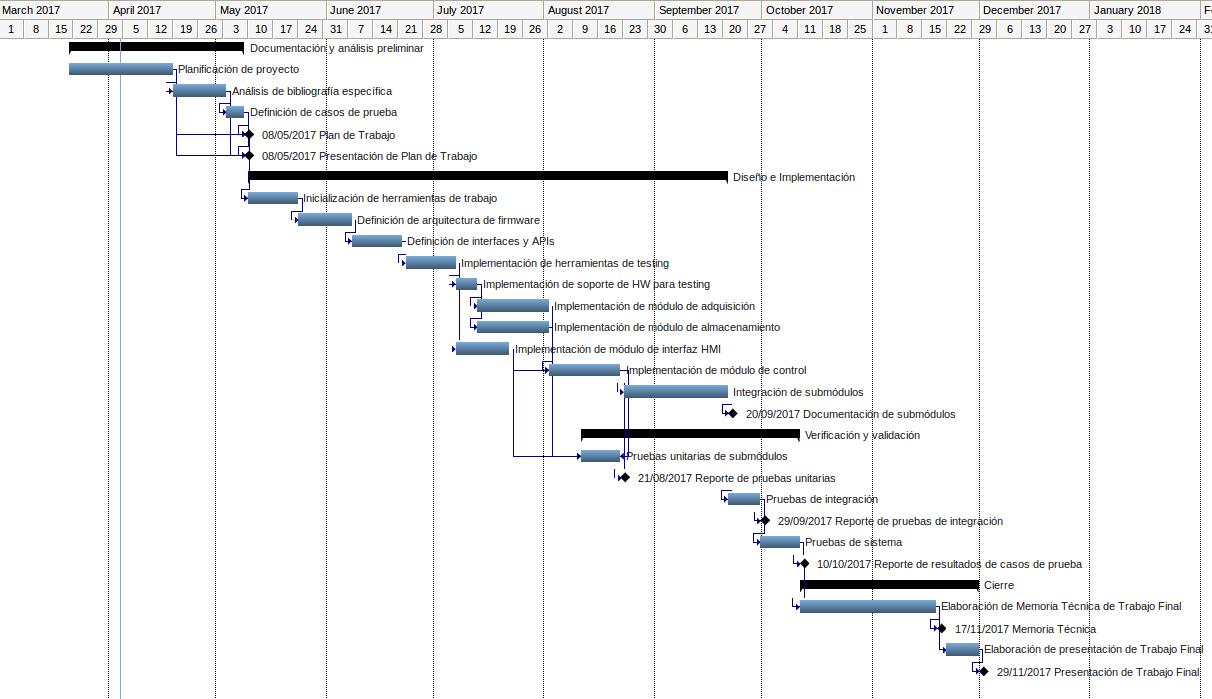
\includegraphics[height=.85\textheight]{./Figuras/Gantt-2.png}
\caption{Ejemplo de diagrama de Gantt (apaisado).} %Modificar este título acorde.
\label{fig:diagGantt}
\end{figure}

\end{landscape}

\end{consigna}


\section{12. Presupuesto detallado del proyecto}
\label{sec:presupuesto}

\begin{consigna}{red}
Si el proyecto es complejo entonces separarlo en partes:
\begin{itemize}
	\item Un total global, indicando el subtotal acumulado por cada una de las áreas.
	\item El desglose detallado del subtotal de cada una de las áreas.
\end{itemize}

IMPORTANTE: No olvidarse de considerar los COSTOS INDIRECTOS.

Incluir la aclaración de si se emplea como moneda el peso argentino (ARS) o si se usa moneda extranjera (USD, EUR, etc). Si es en moneda extranjera se debe indicar la tasa de conversión respecto a la moneda local en una fecha dada.

\end{consigna}

\begin{table}[htpb]
\centering
\begin{tabularx}{\linewidth}{@{}|X|c|r|r|@{}}
\hline
\rowcolor[HTML]{C0C0C0} 
\multicolumn{4}{|c|}{\cellcolor[HTML]{C0C0C0}COSTOS DIRECTOS} \\ \hline
\rowcolor[HTML]{C0C0C0} 
Descripción &
  \multicolumn{1}{c|}{\cellcolor[HTML]{C0C0C0}Cantidad} &
  \multicolumn{1}{c|}{\cellcolor[HTML]{C0C0C0}Valor unitario} &
  \multicolumn{1}{c|}{\cellcolor[HTML]{C0C0C0}Valor total} \\ \hline
 &
  \multicolumn{1}{c|}{} &
  \multicolumn{1}{c|}{} &
  \multicolumn{1}{c|}{} \\ \hline
 &
  \multicolumn{1}{c|}{} &
  \multicolumn{1}{c|}{} &
  \multicolumn{1}{c|}{} \\ \hline
\multicolumn{1}{|l|}{} &
   &
   &
   \\ \hline
\multicolumn{1}{|l|}{} &
   &
   &
   \\ \hline
\multicolumn{3}{|c|}{SUBTOTAL} &
  \multicolumn{1}{c|}{} \\ \hline
\rowcolor[HTML]{C0C0C0} 
\multicolumn{4}{|c|}{\cellcolor[HTML]{C0C0C0}COSTOS INDIRECTOS} \\ \hline
\rowcolor[HTML]{C0C0C0} 
Descripción &
  \multicolumn{1}{c|}{\cellcolor[HTML]{C0C0C0}Cantidad} &
  \multicolumn{1}{c|}{\cellcolor[HTML]{C0C0C0}Valor unitario} &
  \multicolumn{1}{c|}{\cellcolor[HTML]{C0C0C0}Valor total} \\ \hline
\multicolumn{1}{|l|}{} &
   &
   &
   \\ \hline
\multicolumn{1}{|l|}{} &
   &
   &
   \\ \hline
\multicolumn{1}{|l|}{} &
   &
   &
   \\ \hline
\multicolumn{3}{|c|}{SUBTOTAL} &
  \multicolumn{1}{c|}{} \\ \hline
\rowcolor[HTML]{C0C0C0}
\multicolumn{3}{|c|}{TOTAL} &
   \\ \hline
\end{tabularx}%
\end{table}


\section{13. Gestión de riesgos}
\label{sec:riesgos}

\begin{consigna}{red}
a) Identificación de los riesgos (al menos cinco) y estimación de sus consecuencias:
 
Riesgo 1: detallar el riesgo (riesgo es algo que si ocurre altera los planes previstos de forma negativa)
\begin{itemize}
	\item Severidad (S): mientras más severo, más alto es el número (usar números del 1 al 10).\\
	Justificar el motivo por el cual se asigna determinado número de severidad (S).
	\item Probabilidad de ocurrencia (O): mientras más probable, más alto es el número (usar del 1 al 10).\\
	Justificar el motivo por el cual se asigna determinado número de (O). 
\end{itemize}   

Riesgo 2:
\begin{itemize}
	\item Severidad (S): X.\\
	Justificación...
	\item Ocurrencia (O): Y.\\
	Justificación...
\end{itemize}

Riesgo 3:
\begin{itemize}
	\item Severidad (S):  X.\\
	Justificación...
	\item Ocurrencia (O): Y.\\
	Justificación...
\end{itemize}


b) Tabla de gestión de riesgos:      (El RPN se calcula como RPN=SxO)

\begin{table}[htpb]
\centering
\begin{tabularx}{\linewidth}{@{}|X|c|c|c|c|c|c|@{}}
\hline
\rowcolor[HTML]{C0C0C0} 
Riesgo & S & O & RPN & S* & O* & RPN* \\ \hline
       &   &   &     &    &    &      \\ \hline
       &   &   &     &    &    &      \\ \hline
       &   &   &     &    &    &      \\ \hline
       &   &   &     &    &    &      \\ \hline
       &   &   &     &    &    &      \\ \hline
\end{tabularx}%
\end{table}

Criterio adoptado: 

Se tomarán medidas de mitigación en los riesgos cuyos números de RPN sean mayores a...

Nota: los valores marcados con (*) en la tabla corresponden luego de haber aplicado la mitigación.

c) Plan de mitigación de los riesgos que originalmente excedían el RPN máximo establecido:
 
Riesgo 1: plan de mitigación (si por el RPN fuera necesario elaborar un plan de mitigación).
  Nueva asignación de S y O, con su respectiva justificación:
  \begin{itemize}
	\item Severidad (S*): mientras más severo, más alto es el número (usar números del 1 al 10).
          Justificar el motivo por el cual se asigna determinado número de severidad (S).
	\item Probabilidad de ocurrencia (O*): mientras más probable, más alto es el número (usar del 1 al 10).
          Justificar el motivo por el cual se asigna determinado número de (O).
	\end{itemize}

Riesgo 2: plan de mitigación (si por el RPN fuera necesario elaborar un plan de mitigación).
 
Riesgo 3: plan de mitigación (si por el RPN fuera necesario elaborar un plan de mitigación).

\end{consigna}


\section{14. Gestión de la calidad}
\label{sec:calidad}

\begin{consigna}{red}
Elija al menos diez requerimientos que a su criterio sean los más importantes/críticos/que aportan más valor y para cada uno de ellos indique las acciones de verificación y validación que permitan asegurar su cumplimiento.

\begin{itemize} 
\item Req \#1: copiar acá el requerimiento con su correspondiente número.

\begin{itemize}
	\item Verificación para confirmar si se cumplió con lo requerido antes de mostrar el sistema al cliente. Detallar.
	\item Validación con el cliente para confirmar que está de acuerdo en que se cumplió con lo requerido. Detallar. 
\end{itemize}

\end{itemize}

Tener en cuenta que en este contexto se pueden mencionar simulaciones, cálculos, revisión de hojas de datos, consulta con expertos, mediciones, etc.  

Las acciones de verificación suelen considerar al entregable como ``caja blanca'', es decir se conoce en profundidad su funcionamiento interno.  

En cambio, las acciones de validación suelen considerar al entregable como ``caja negra'', es decir, que no se conocen los detalles de su funcionamiento interno.

\end{consigna}

\section{15. Procesos de cierre}    
\label{sec:cierre}

\begin{consigna}{red}
Establecer las pautas de trabajo para realizar una reunión final de evaluación del proyecto, tal que contemple las siguientes actividades:

\begin{itemize}
	\item Pautas de trabajo que se seguirán para analizar si se respetó el Plan de Proyecto original:\\
	 - Indicar quién se ocupará de hacer esto y cuál será el procedimiento a aplicar. 
	\item Identificación de las técnicas y procedimientos útiles e inútiles que se emplearon, los problemas que surgieron y cómo se solucionaron:\\
	 - Indicar quién se ocupará de hacer esto y cuál será el procedimiento para dejar registro.
	\item Indicar quién organizará el acto de agradecimiento a todos los interesados, y en especial al equipo de trabajo y colaboradores:\\
	  - Indicar esto y quién financiará los gastos correspondientes.
\end{itemize}

\end{consigna}

\end{document}